\documentclass{../template/tp}
\usepackage[utf8x]{inputenc}

\usepackage[english]{babel}
\usepackage[T1]{fontenc}

\usepackage{graphicx}
\usepackage{amssymb}
\usepackage{amsmath}
\usepackage{wasysym} %smiley
\usepackage{hyperref}% hyperliens
\usepackage{tikz}
\usetikzlibrary{babel,positioning,calc}
\usepackage[]{circuitikz}
\usepackage{textcomp}
% \usepackage{minted}
\usepackage[long]{datetime}
\usepackage{gensymb} % \ohm, celsius
\usepackage{framed}
\usepackage{pdfpages}
\usepackage{todonotes}
\usepackage{enumitem}
\usepackage{ marvosym }
\usepackage{qrcode}%Don't forget to escape the "#", as the href package requires.
\usepackage{tabularx}

\usepackage{mathastext} % math as standfard text : units are respecting typography conventions.
\usepackage{fancyhdr}
% \langexam{frenchb}

\usepackage{subcaption}

\graphicspath{{imgs/}}

\newcommand{\labTitle}{Ladder Diagrams \& GRAFCET}
\newcommand{\labNumber}{2}

\newcommand{\version}{v1.0.0}

\newcommand{\mnemonic}{ELEC-H-516}
\newcommand{\courseName}{Programmable Logic Controllers}

\newboolean{koriG}
\ifx\koriG\undefined
\correction{false}
\else
\correction{true}
\fi

% \correction{false}
% \correction{true}

\author{The Fantastic Four}


%% fancy header & foot
\pagestyle{fancy}
\lhead{[\mnemonic] \courseName\\ LABO  \labNumber :  \labTitle}
\rhead{\version\\ page \thepage}
\cfoot{}
%%

\pdfinfo{
/Author (ULB -- BEAMS)
/Title (Labo \labNumber \mnemonic, \labTitle)
/ModDate (D:\pdfdate)

}
\hypersetup{
pdftitle={Labo \labNumber [\mnemonic] \courseName : \labTitle},
pdfauthor={©2017 ULB - BEAMS  },
pdfsubject={\labTitle}
}


\setlength{\parskip}{0.5cm plus4mm minus3mm} %espacement entre §
\setlength{\parindent}{0pt}

\begin{document}

\tptitle{}{Labo \labNumber : \labTitle}

\vspace{-1cm}

\rule{\linewidth}{.5pt}

The activation of the GRAFCET step can be represented in the Ladder diagram using
one sequential memory block (SR) : 0 indicating that the state is not active and 1 when it
is active. The synthesis of such specification consists in determining the control functions of
the SR FF.

\Question{
	Construct a linear GRAFCET with 5 different steps using Ladder Diagram. Choose inputs and actions freely.
}{}

\Question{
	Using ladder diagrams construct the problem for a GRAFCET shown on Figure~\ref{grafcet}: Choose inputs and actions freely.
	\begin{figure}[h]
		\centering
		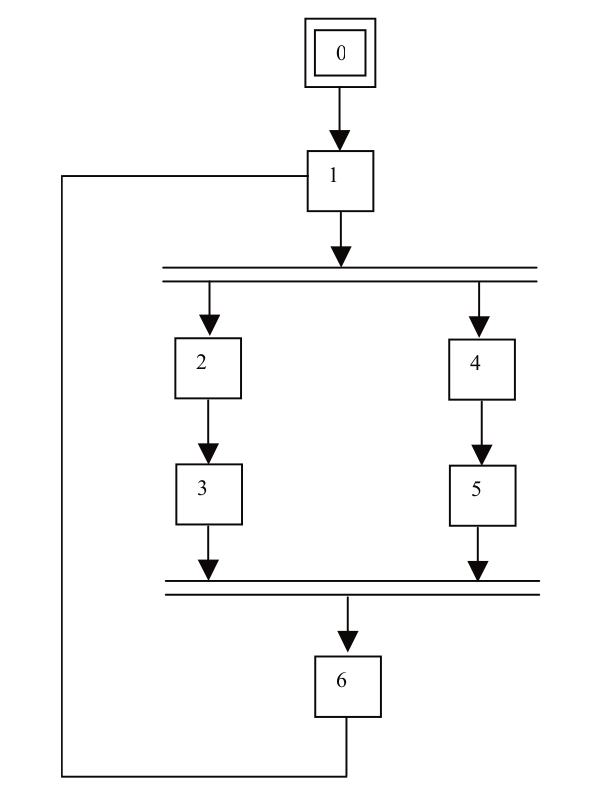
\includegraphics[width=0.4\linewidth]{grafcet}
		\caption{GRAFCET to be made using Ladder diagram.}
		\label{grafcet}
	\end{figure}
}{}

\Question{
	Implement a traffic light using GRAFCET (SFC). 
	First build a single traffic light that will switch between green, orange and red automatically using timers.
    Then add a second one that controls a perpendicular road. They thus can't be green at the same time.
}{}


\end{document}